\documentclass[handout]{beamer}

\usepackage{graphicx}
\usepackage{tikz-cd}

\title{EPIT Lecture 5.3\\ Homotopical constructions of types}
\author{Egbert Rijke}
\date{Friday, April 16th 2020}

\setbeamertemplate{caption}{\raggedright\insertcaption\par}

\mathchardef\usc="2D
\newcommand{\N}{\mathbb{N}}
\newcommand{\Z}{\mathbb{Z}}
\newcommand{\UU}{\mathcal{U}}
\newcommand{\brck}[1]{\|#1\|}
\newcommand{\Brck}[1]{\left\|#1\right\|}
\newcommand{\trunc}[2]{\|#2\|_{#1}}
\newcommand{\Trunc}[2]{\left\|#2\right\|_{#1}}
\newcommand{\unit}{\mathbf{1}}
\newcommand{\sphere}[1]{S^{#1}}
\newcommand{\isnull}{\mathsf{is\usc{}null}}
\newcommand{\htpy}{\sim}
\newcommand{\apbinary}{\mathsf{ap\usc{}bin}}
\newcommand{\Glob}{\mathsf{Glob}}
\newcommand{\typeGlob}{\mathsf{type}}
\newcommand{\relGlob}{\mathsf{rel}}
\newcommand{\homGlob}{\mathsf{hom}}
\newcommand{\maphomGlob}{\mathsf{map}}
\newcommand{\cgrhomGlob}{\mathsf{cgr}}
\newcommand{\bihomGlob}{\mathsf{bihom}}
\newcommand{\mapbihomGlob}{\mathsf{map}}
\newcommand{\cgrbihomGlob}{\mathsf{cgr}}
\newcommand{\ct}{\bullet}
\newcommand{\isconstant}[2]{\mathsf{is\usc{}}(#1,#2)\mathsf{\usc{}constant}}
\newcommand{\ap}{\mathsf{ap}}
\newcommand{\interchange}{\mathsf{interchange}}
\newcommand{\refl}{\mathsf{refl}}
\newcommand{\eh}{\mathsf{eckmann\usc{}hilton}}
\newcommand{\blank}{\mathord{\hspace{1pt}\text{--}\hspace{1pt}}}
\newcommand{\EM}{\mathsf{EM}}
\newcommand{\baseS}{\mathsf{base}}
\newcommand{\loopS}{\mathsf{loop}}
\newcommand{\apd}{\mathsf{apd}}
\newcommand{\tr}{\mathsf{tr}}
\newcommand{\idfunc}{\mathsf{id}}
\newcommand{\mulcircle}{\mu}
\newcommand{\basemulcircle}{\mathsf{base\usc{}mul}_{\sphere{1}}}
\newcommand{\loopmulcircle}{\mathsf{loop\usc{}mul}_{\sphere{1}}}
\newcommand{\htpyidcircle}{H}
\newcommand{\basehtpyidcircle}{\alpha}
\newcommand{\loophtpyidcircle}{\beta}
\newcommand{\invcircle}{\mathsf{inv}_{\sphere{1}}}
\newcommand{\evbase}{\mathsf{ev\usc{}base}}
\newcommand{\eqhtpy}{\mathsf{eq\usc{}htpy}}
\newcommand{\apply}[2]{#1(#2)}
\newcommand{\equiveq}{\mathsf{equiv\usc{}eq}}
\newcommand{\succZ}{\mathsf{succ}}
\newcommand{\bool}{\mathsf{bool}}
\newcommand{\const}{\mathsf{const}}
\newcommand{\btrue}{\mathsf{true}}
\newcommand{\bfalse}{\mathsf{false}}
\newcommand{\ttt}{\mathsf{pt}}
\newcommand{\inl}{\mathsf{inl}}
\newcommand{\inr}{\mathsf{inr}}
\newcommand{\glue}{\mathsf{glue}}
\newcommand{\fib}{\mathsf{fib}}

\setbeamertemplate{navigation symbols}{}
\setbeamertemplate{footline}[frame number]{}

\begin{document}

\begin{frame}
  \maketitle
\end{frame}

\begin{frame}
  Many spaces in topology are constructed by attaching cells, i.e., they are defined as CW-complexes.
  \begin{example}
    We can define a sphere by gluing the boundary of a disk to a single point.
  \end{example}
  Such constructions satisfy universal properties. In type theory, we can define many of them as higher inductive type.\\[1em]

  In this lecture we will see basic constructions of types such as spheres and suspensions, and we will study their basic properties.
\end{frame}

\begin{frame}
  \frametitle{Homotopy pushouts}
  Given $A \stackrel{f}{\leftarrow} S \stackrel{g}{\rightarrow} B$, the pushout of $f$ and $g$ is a type $A\sqcup^S B$ that fits in a commuting square
  \begin{equation*}
    \begin{tikzcd}[ampersand replacement=\&]
      S \arrow[d,swap,"f"] \arrow[r,"g"] \& B \arrow[d,"\inr"] \\
      A \arrow[r,swap,"\inl"] \& A\sqcup^C B
    \end{tikzcd}
  \end{equation*}
  I.e., it is the higher inductive type generated $A\sqcup^S B$ generated by
  \begin{align*}
    \inl & : A \to A\sqcup^S B \\
    \inr & : B \to A\sqcup^S B \\
    \glue & : \prod_{(s:S)}\inl(f(s))=\inr(g(s)).
  \end{align*}
\end{frame}

\begin{frame}
  The induction principle for the higher inductive type $A\sqcup^S B$ implies the universal property of the pushout: For any type $X$ equipped with
  \begin{align*}
    i & : A \to X \\
    j & : B \to X \\
    H & : i\circ f \sim j\circ g
  \end{align*}
  there is a unique map $h:A\sqcup^S B\to X$ such that the following diagram commutes:
  \begin{equation*}
    \begin{tikzcd}[ampersand replacement=\&]
      S \arrow[d,swap,"f"] \arrow[r,"g"] \& B \arrow[d,swap,"\inr"] \arrow[ddr,bend left=15,"j"] \\
      A \arrow[r,"\inl"] \arrow[drr,bend right=15,swap,"i"] \& A \sqcup^S B \arrow[dr,"h"] \\
      \& \& X
    \end{tikzcd}
  \end{equation*}
\end{frame}

\begin{frame}
  \begin{example}
    The circle fits in a pushout square
    \begin{equation*}
      \begin{tikzcd}[ampersand replacement=\&]
        \mathbf{2} \arrow[r] \arrow[d] \& \mathbf{1} \arrow[d] \\
        \mathbf{1} \arrow[r] \& \sphere{1}
      \end{tikzcd}
    \end{equation*}
    in whith the homotopy $H:\const_\baseS\circ\const_\ttt\htpy\const\baseS\circ\const_\ttt$ is given by
    \begin{align*}
      H(\btrue) & := \loopS \\
      H(\bfalse) & := \refl
    \end{align*}    
  \end{example}
\end{frame}

\begin{frame}
  \begin{example}
    The suspension $\Sigma X$ of a type $X$ is the pushout
    \begin{equation*}
      \begin{tikzcd}[ampersand replacement=\&]
        X \arrow[r] \arrow[d] \& \unit \arrow[d,"S"] \\
        \unit \arrow[r,swap,"N"] \& \Sigma X.
      \end{tikzcd}
    \end{equation*}
    In other words, the type $\Sigma X$ is the higher inductive type generated by
    \begin{align*}
      N,S & : \Sigma X \\
      \glue & : X\to (N=S).
    \end{align*}
  \end{example}
\end{frame}

\begin{frame}
  \frametitle{A picture of the suspension}
  \begin{center}
    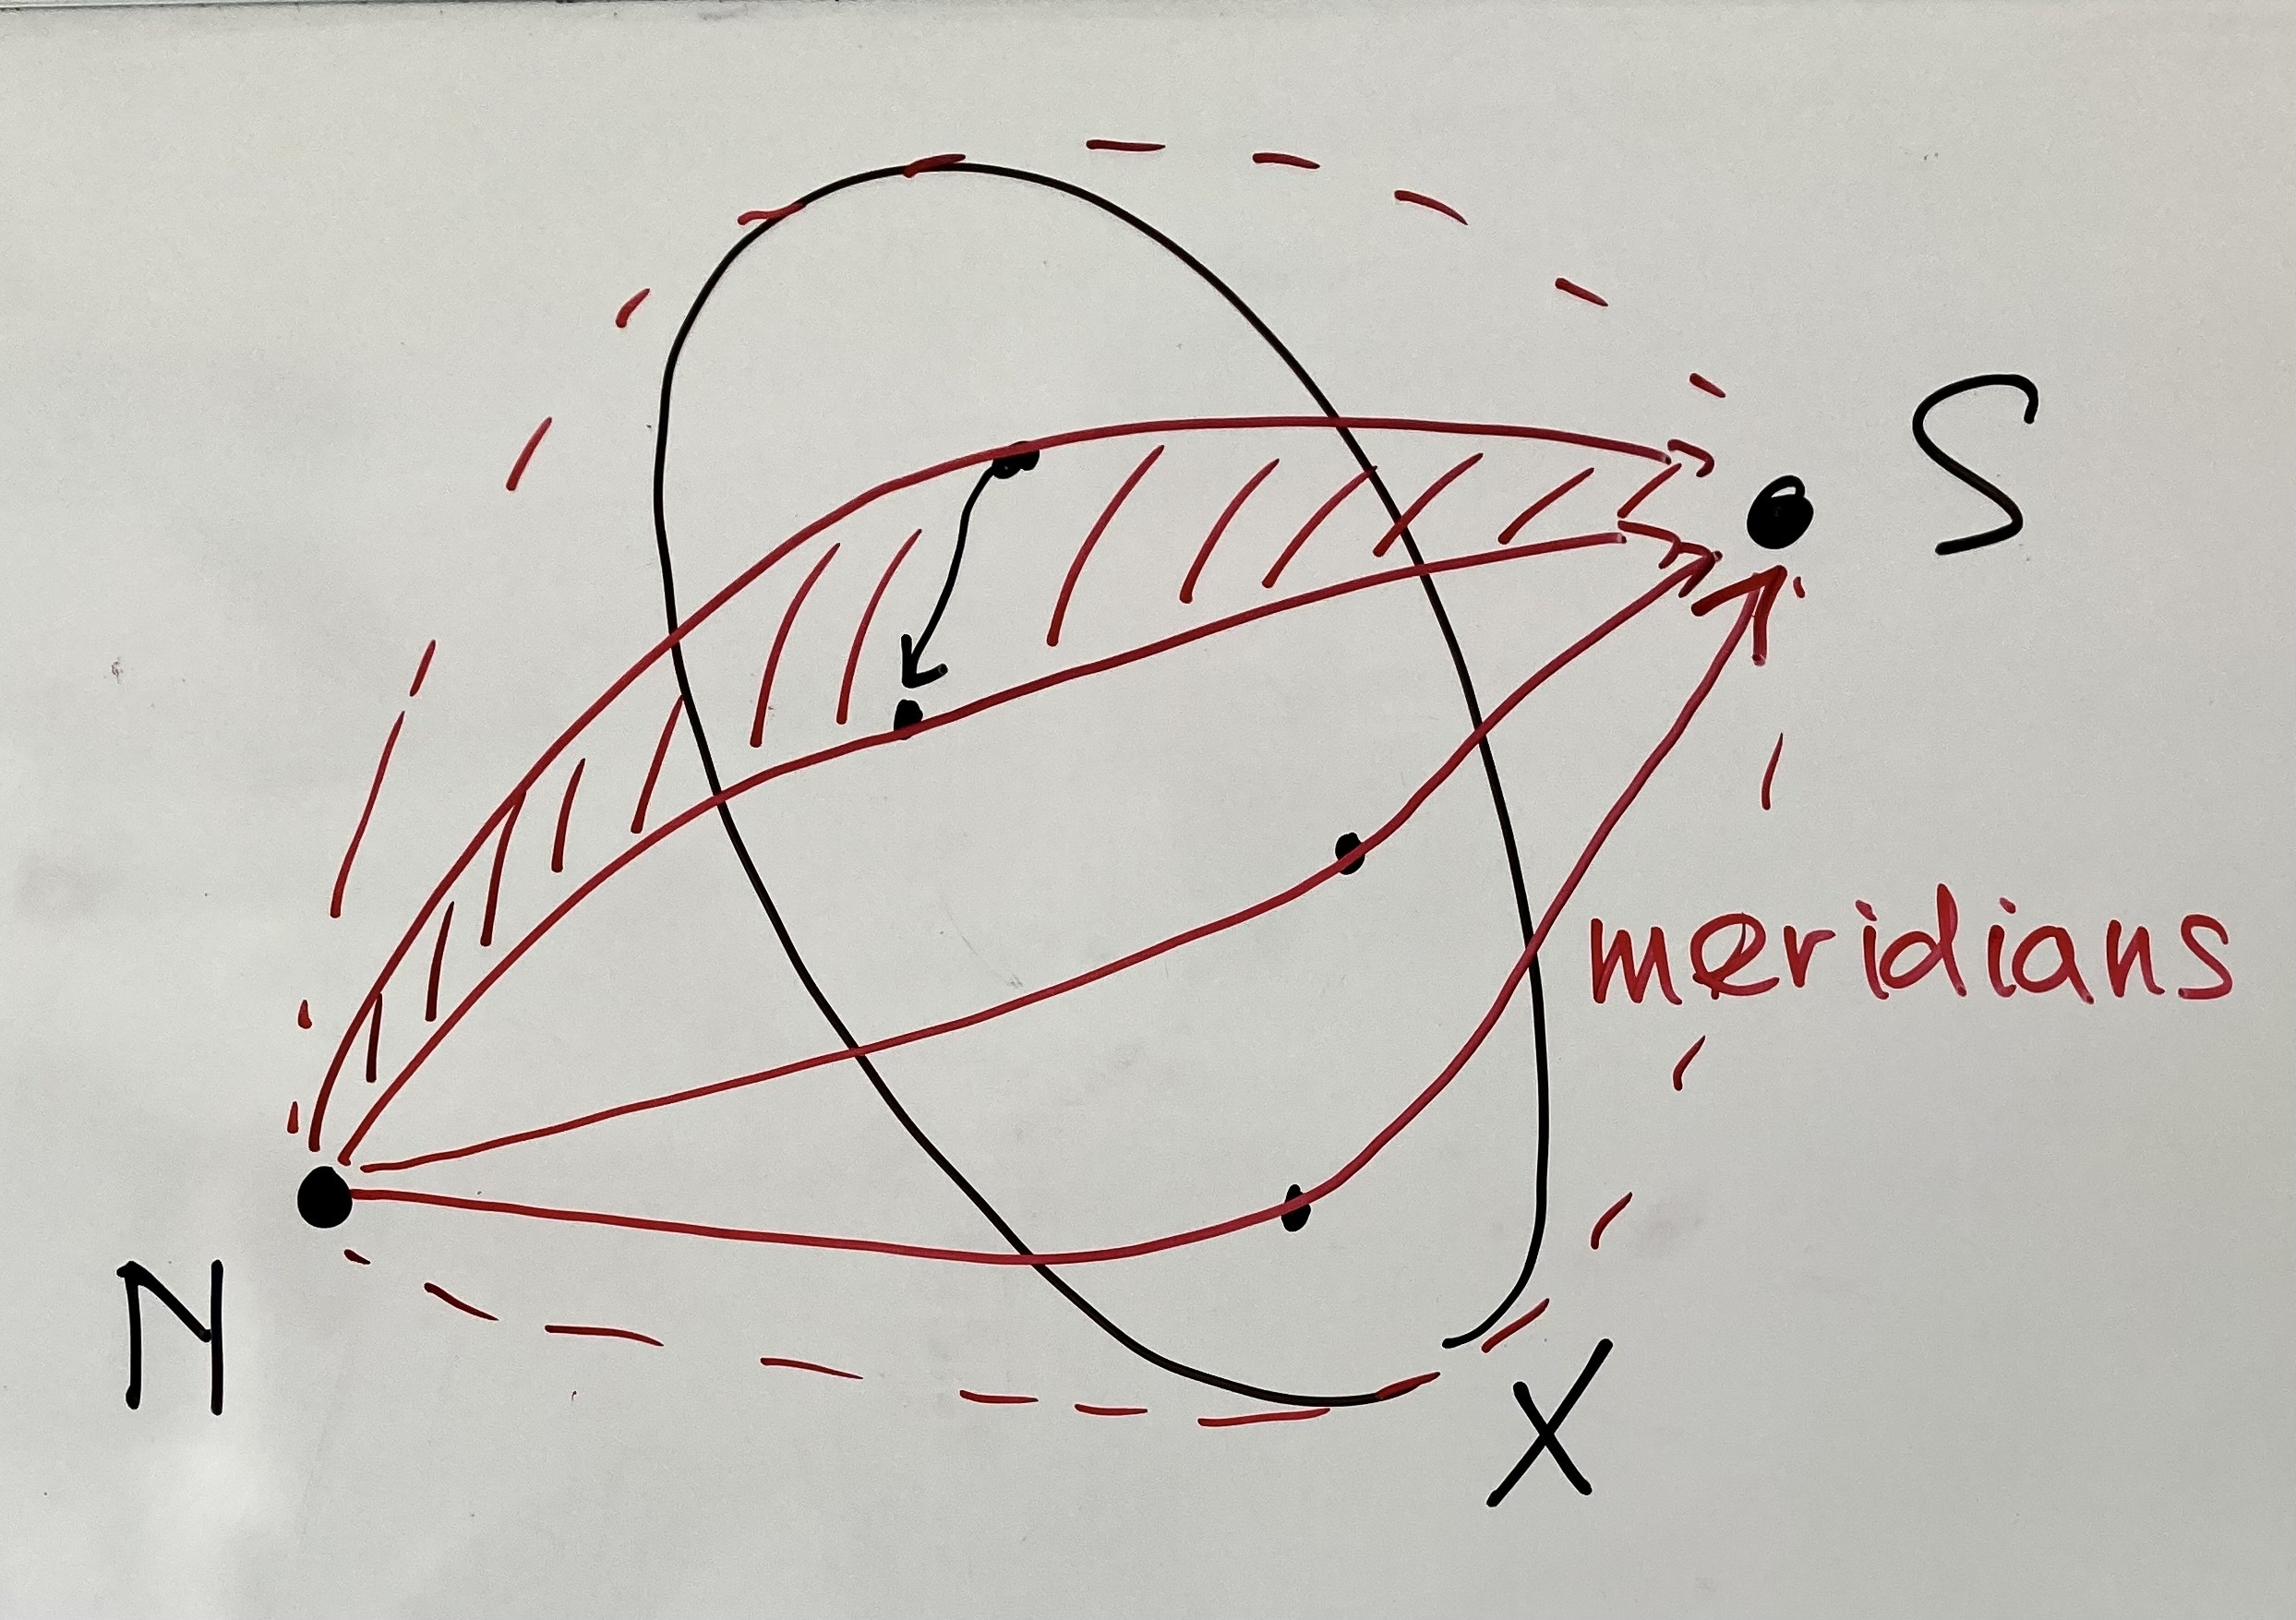
\includegraphics[width=\textwidth]{suspension}
  \end{center}
\end{frame}

\begin{frame}
  \frametitle{The suspension-loop space adjunction}
  \begin{definition}
    Let $X$ and $Y$ be types equipped with points $x_0$ and $y_0$. We define the type of \textbf{pointed maps}
    \begin{equation*}
      (X\to_\ast Y):=\sum\nolimits_{(f:X\to Y)}f(x_0)=y_0.
    \end{equation*}
  \end{definition}

  \begin{definition}
    Let $X$ be a type equipped with a point $x_0$. Then we define
    \begin{equation*}
      \Omega(X,x_0):= x_0=x_0.
    \end{equation*}
    This type comes equipped with the point $\refl:\Omega(X,x)$. 
  \end{definition}
  
  \begin{theorem}
    Let $X$ be a type equipped with a point $x_0$. Then we have an equivalence
    \begin{equation*}
      (\Sigma X\to_\ast Y)\simeq (X\to_\ast\Omega Y)
    \end{equation*}
  \end{theorem}
\end{frame}

\begin{frame}
  \begin{proof}
    \begin{align*}
      (\Sigma X \to_\ast Y)
      & \doteq \sum_{(f:\Sigma X\to Y)}f(N)=y_0 \\ \pause
      & \simeq \sum_{(y,y':Y)}(h:X\to y=y')\times (y=y_0) \\ \pause
      & \simeq \sum_{(y':Y)}(h:X\to y_0=y') \\ \pause
      & \simeq \sum_{(y':Y)}\sum_{(p:y_0=y')}\sum_{(h:X\to y_0=y')}h(x_0)=\refl \\ \pause
      & \simeq \sum_{(h:X\to y_0=y_0)}h(x_0)=\refl \\ \pause
      & \doteq X\to_\ast \Omega Y\qedhere
    \end{align*}
  \end{proof}
\end{frame}

\begin{frame}
    \begin{definition}
    The spheres are defined recursively by
    \begin{align*}
      \sphere{0} & := \mathbf{2} \\
      \sphere{n+1} & :=\Sigma\sphere{n}.
    \end{align*}
  \end{definition}

  \begin{theorem}
    Let $X$ be a pointed type. Then we have
    \begin{equation*}
      (\sphere{n}\to_\ast X)\simeq \Omega^n(X).
    \end{equation*}
  \end{theorem}
\end{frame}

\begin{frame}
  \begin{definition}
    The join $A\ast B$ of two types $A$ and $B$ is defined as the pushout
    \begin{equation*}
      \begin{tikzcd}[ampersand replacement=\&]
        A\times B \arrow[d,"\pi_1"] \arrow[r,"\pi_2"] \& B \arrow[d,"\inr"] \\
        A \arrow[r,swap,"\inl"] \& A\ast B
      \end{tikzcd}
    \end{equation*}
    In other words, $A\ast B$ is the higher inductive type with
    \begin{align*}
      \inl & : A \to A \ast B \\
      \inr & : B \to A \ast B \\
      \glue & : \prod_{(a:A)}\prod_{(b : B)}\inl(a)=\inr(b).
    \end{align*}
  \end{definition}
\end{frame}

\begin{frame}
  \frametitle{A picture of the join}
  \begin{center}
    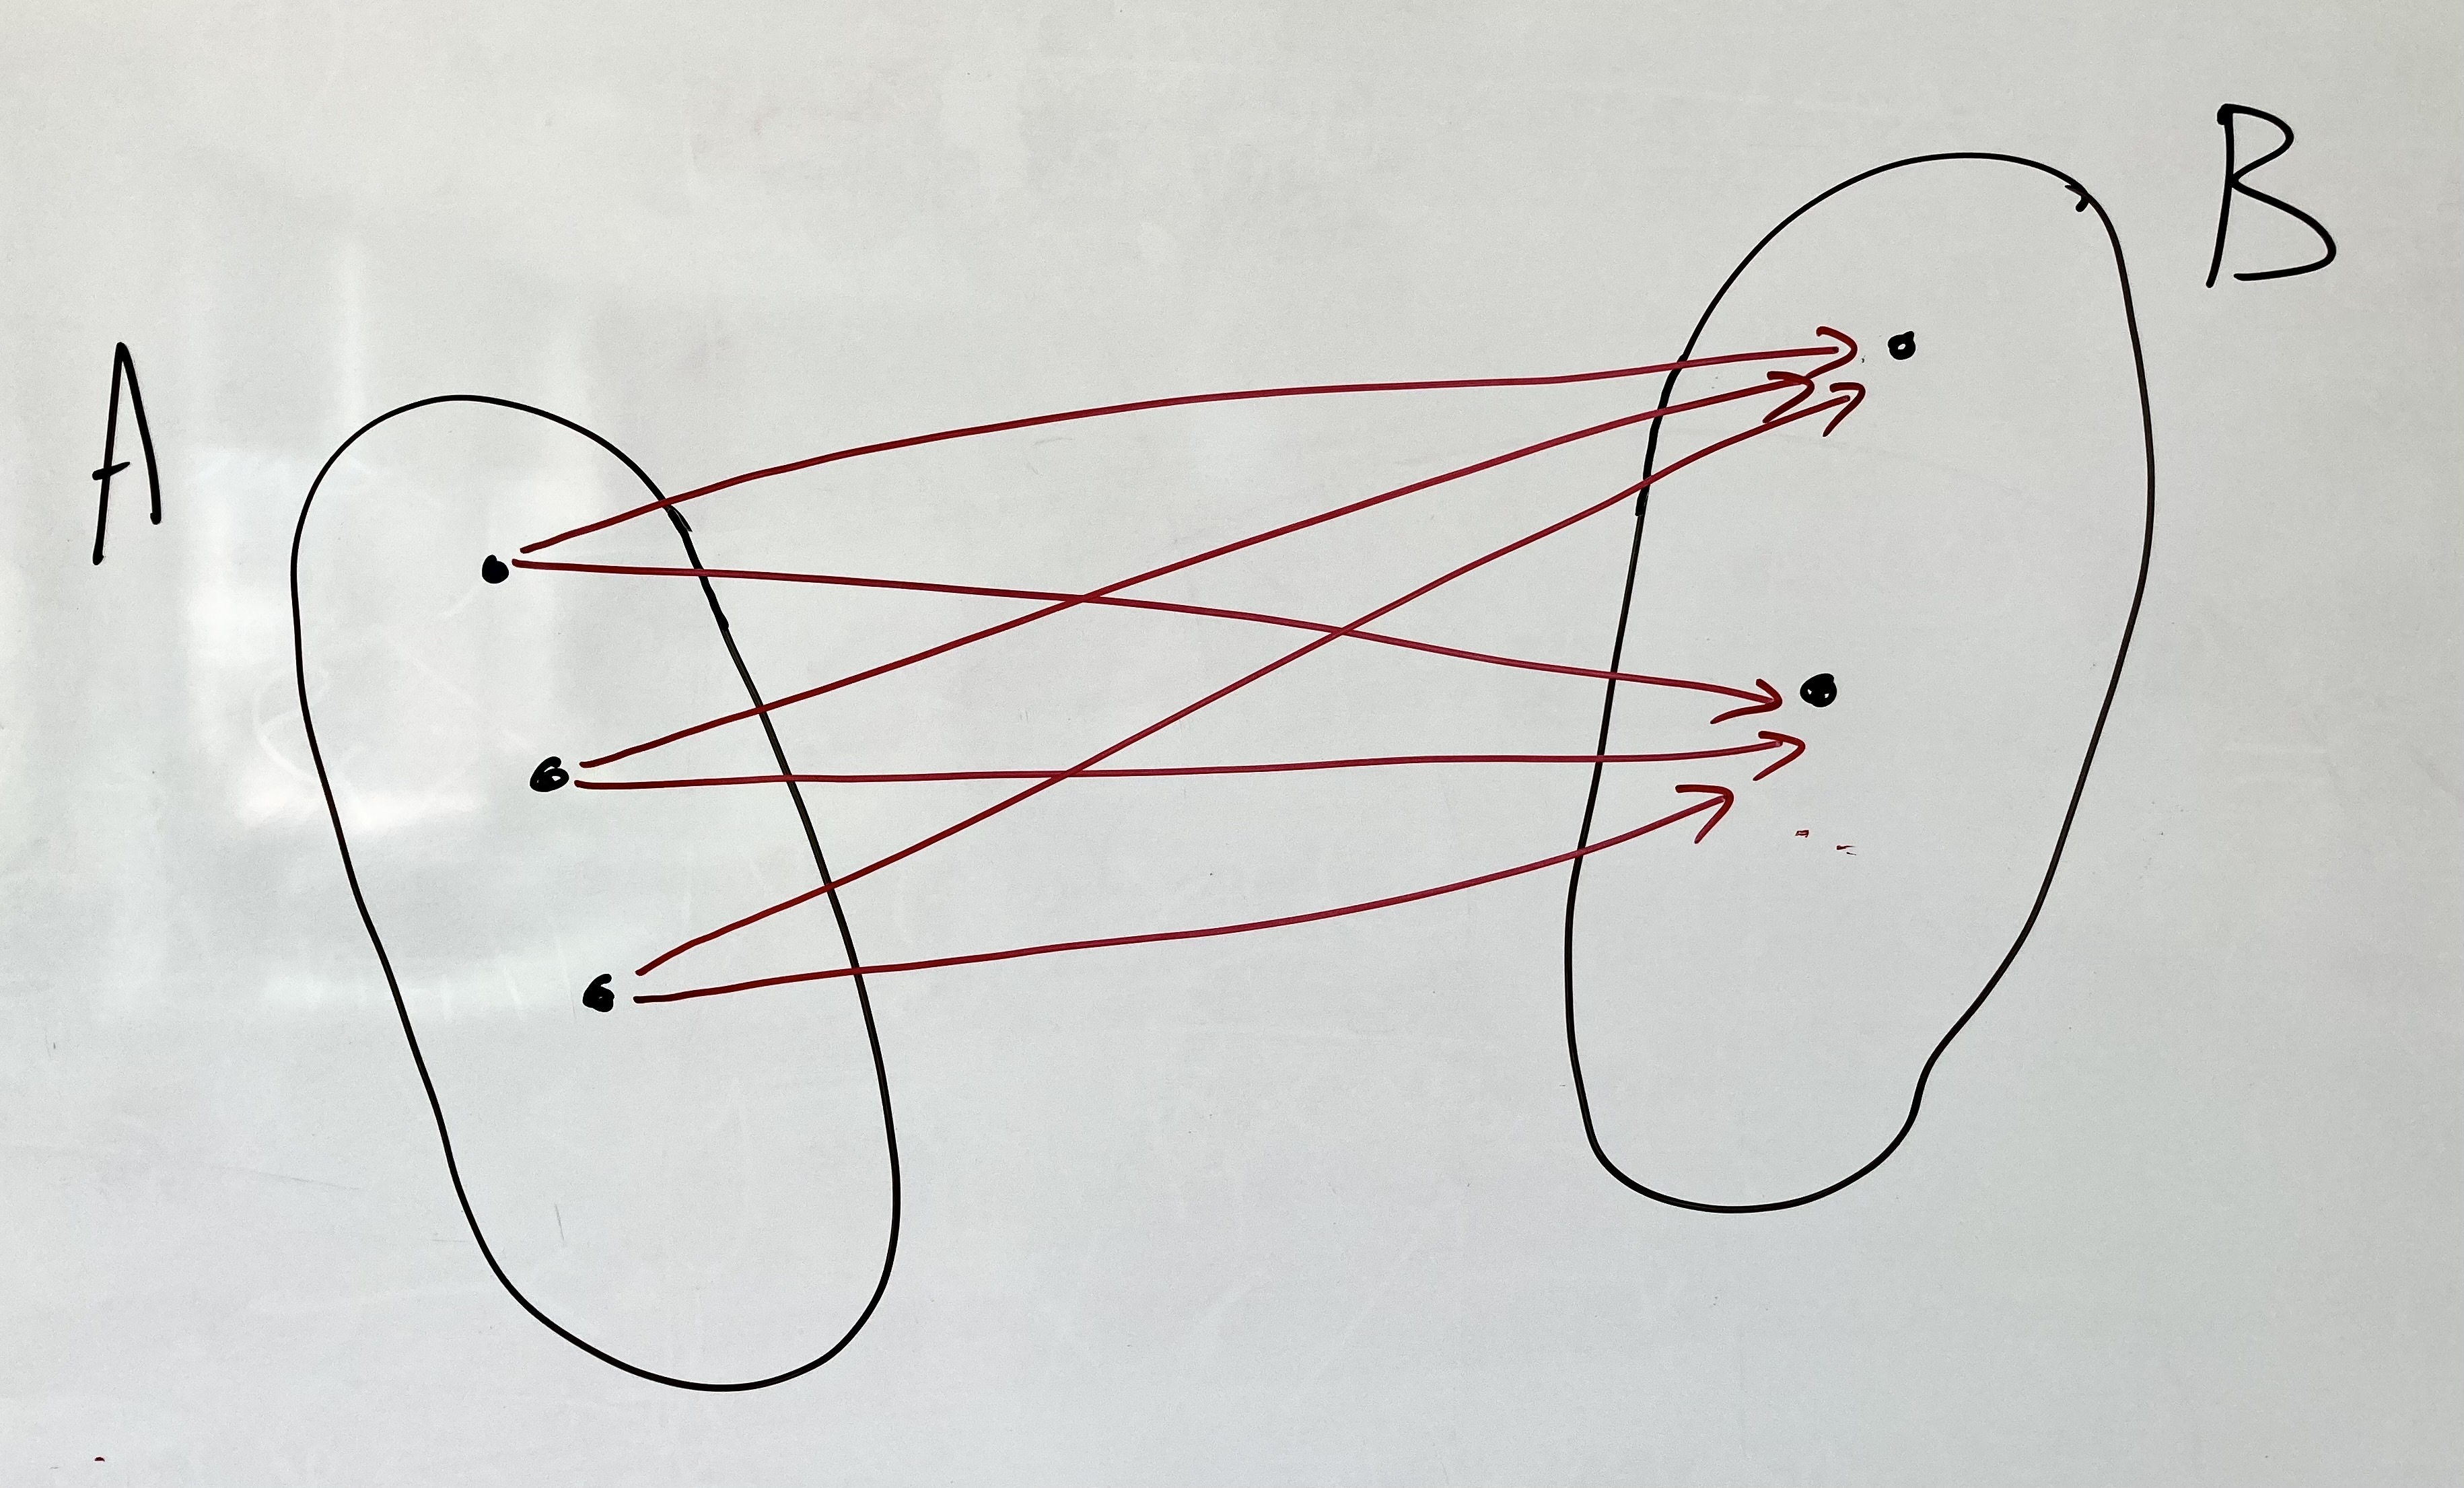
\includegraphics[width=\textwidth]{join}
  \end{center}
\end{frame}

\begin{frame}
  \begin{theorem}
    There is an equivalence $\mathbf{2}\ast X\simeq \Sigma X$.
  \end{theorem}

  \begin{center}
    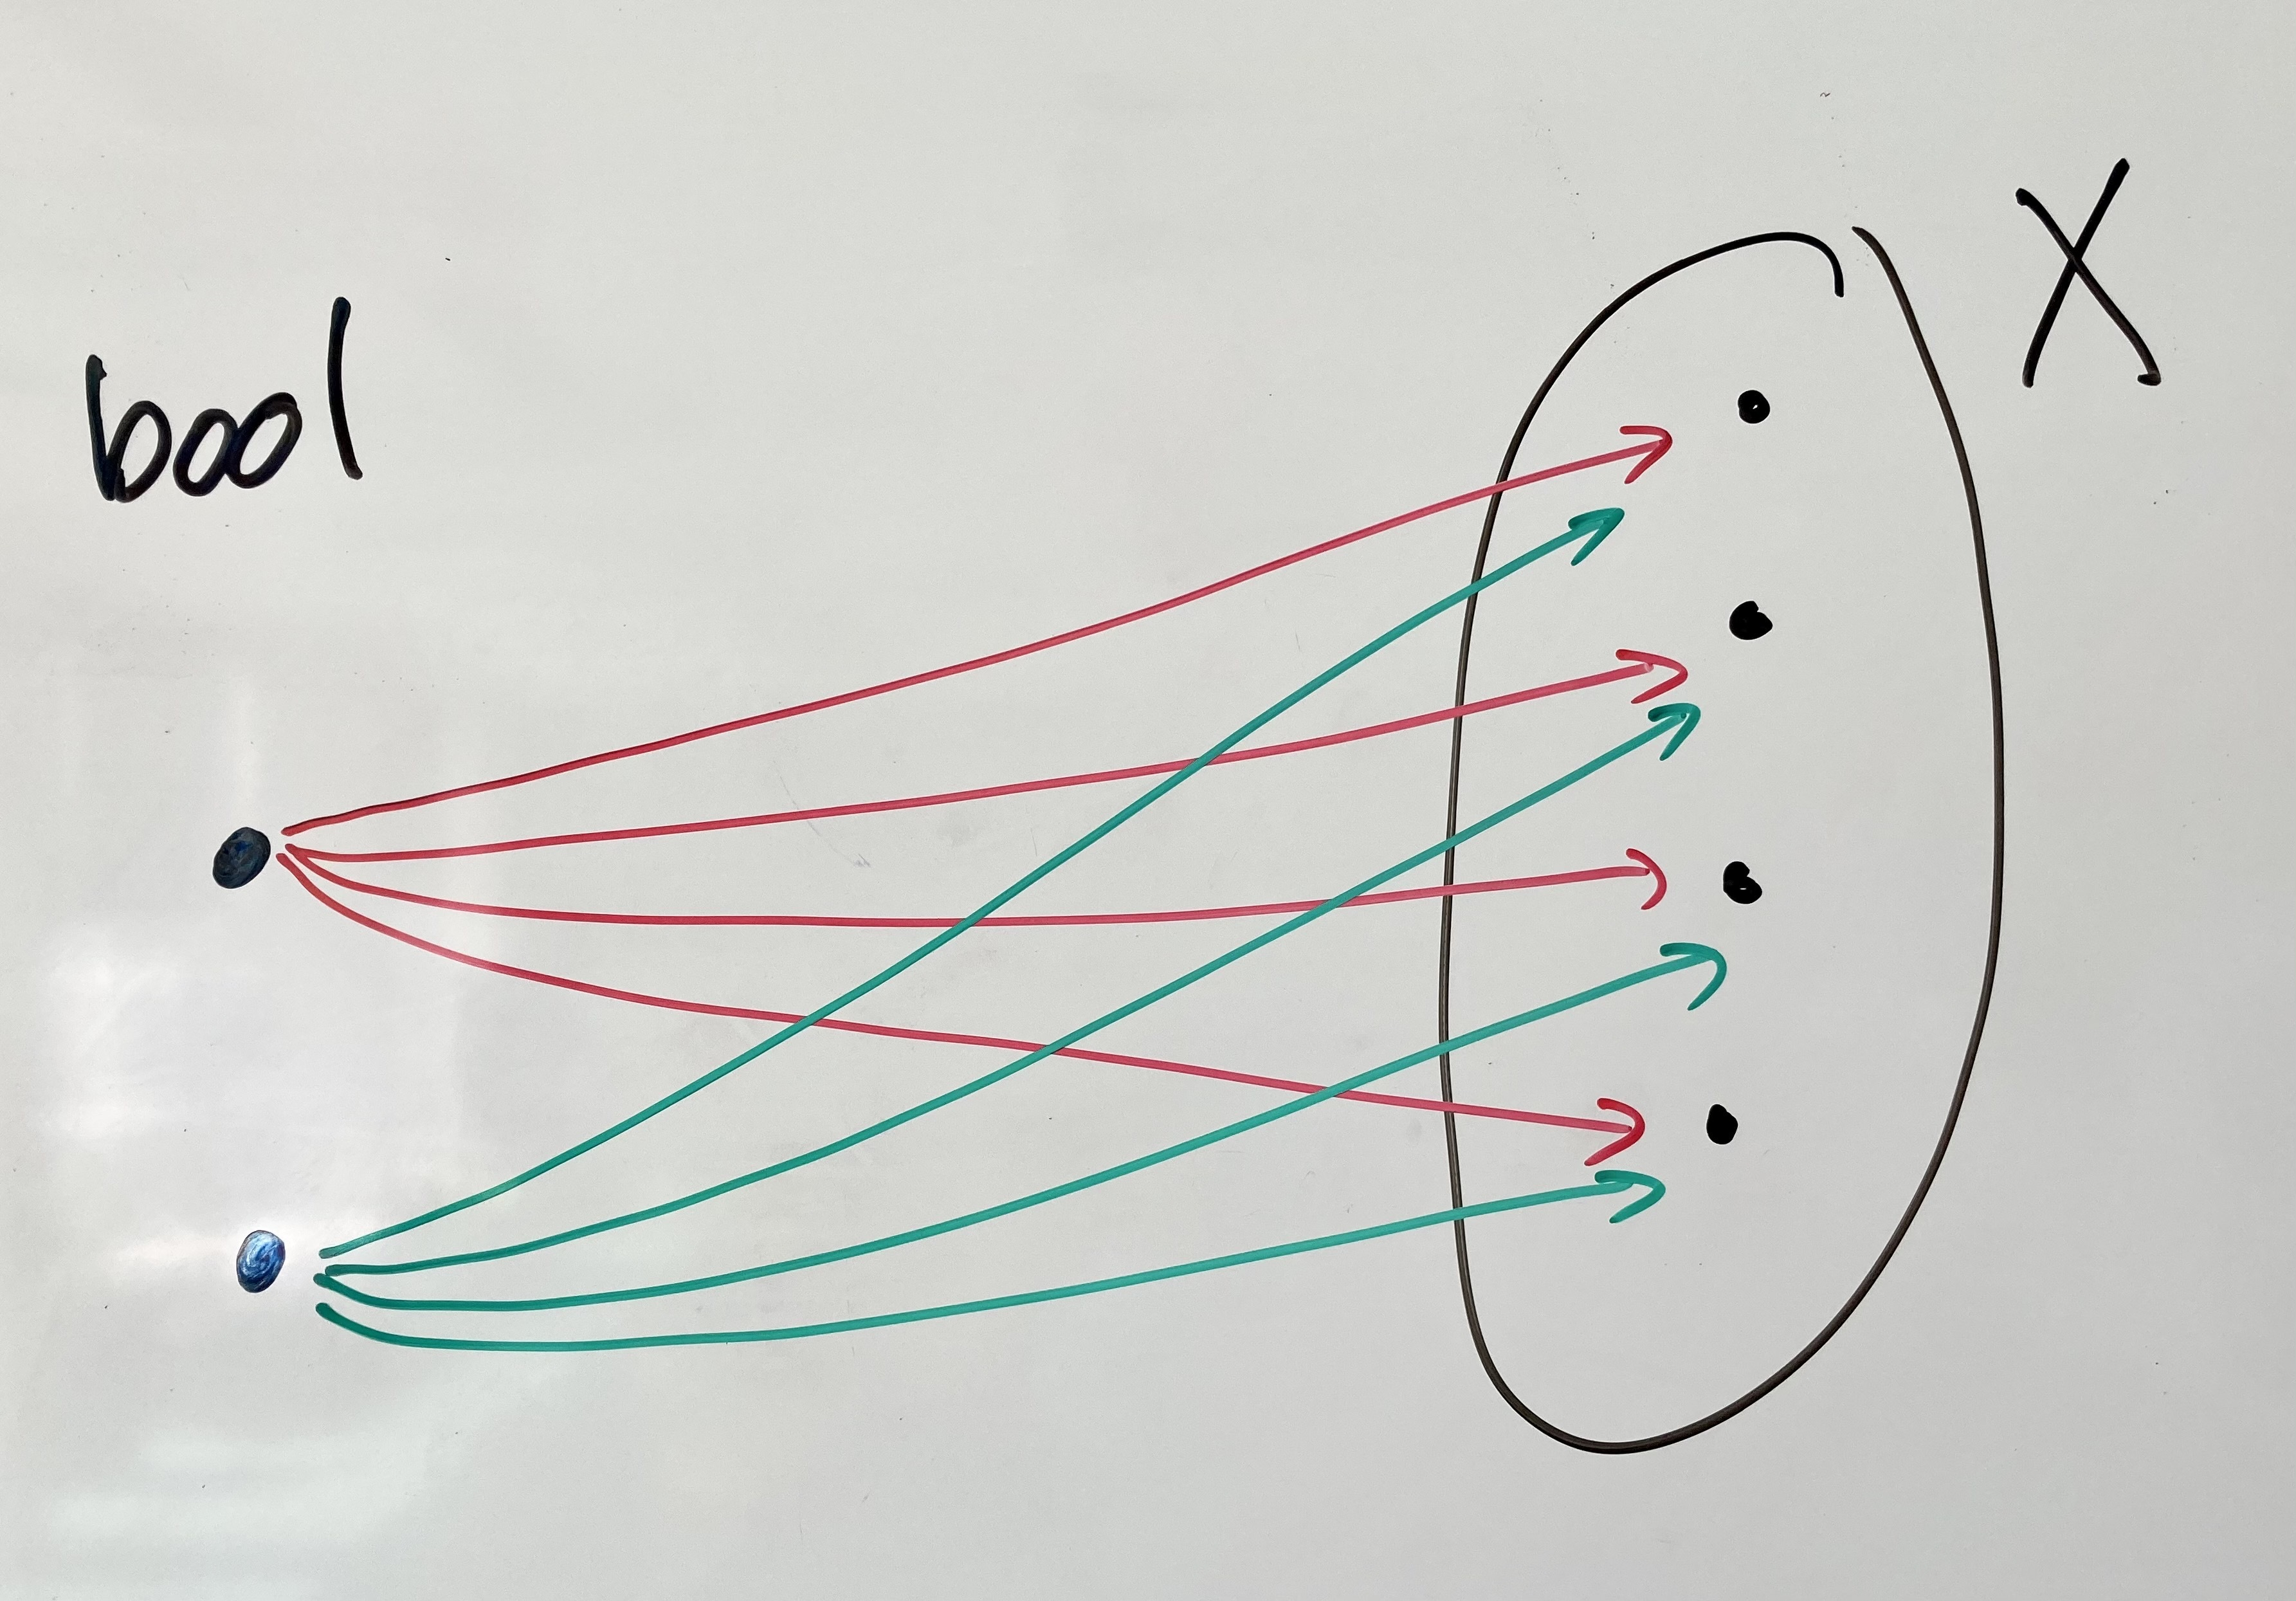
\includegraphics[width=.7\textwidth]{suspension-from-join-1}
  \end{center}
\end{frame}

\begin{frame}
  \begin{center}
    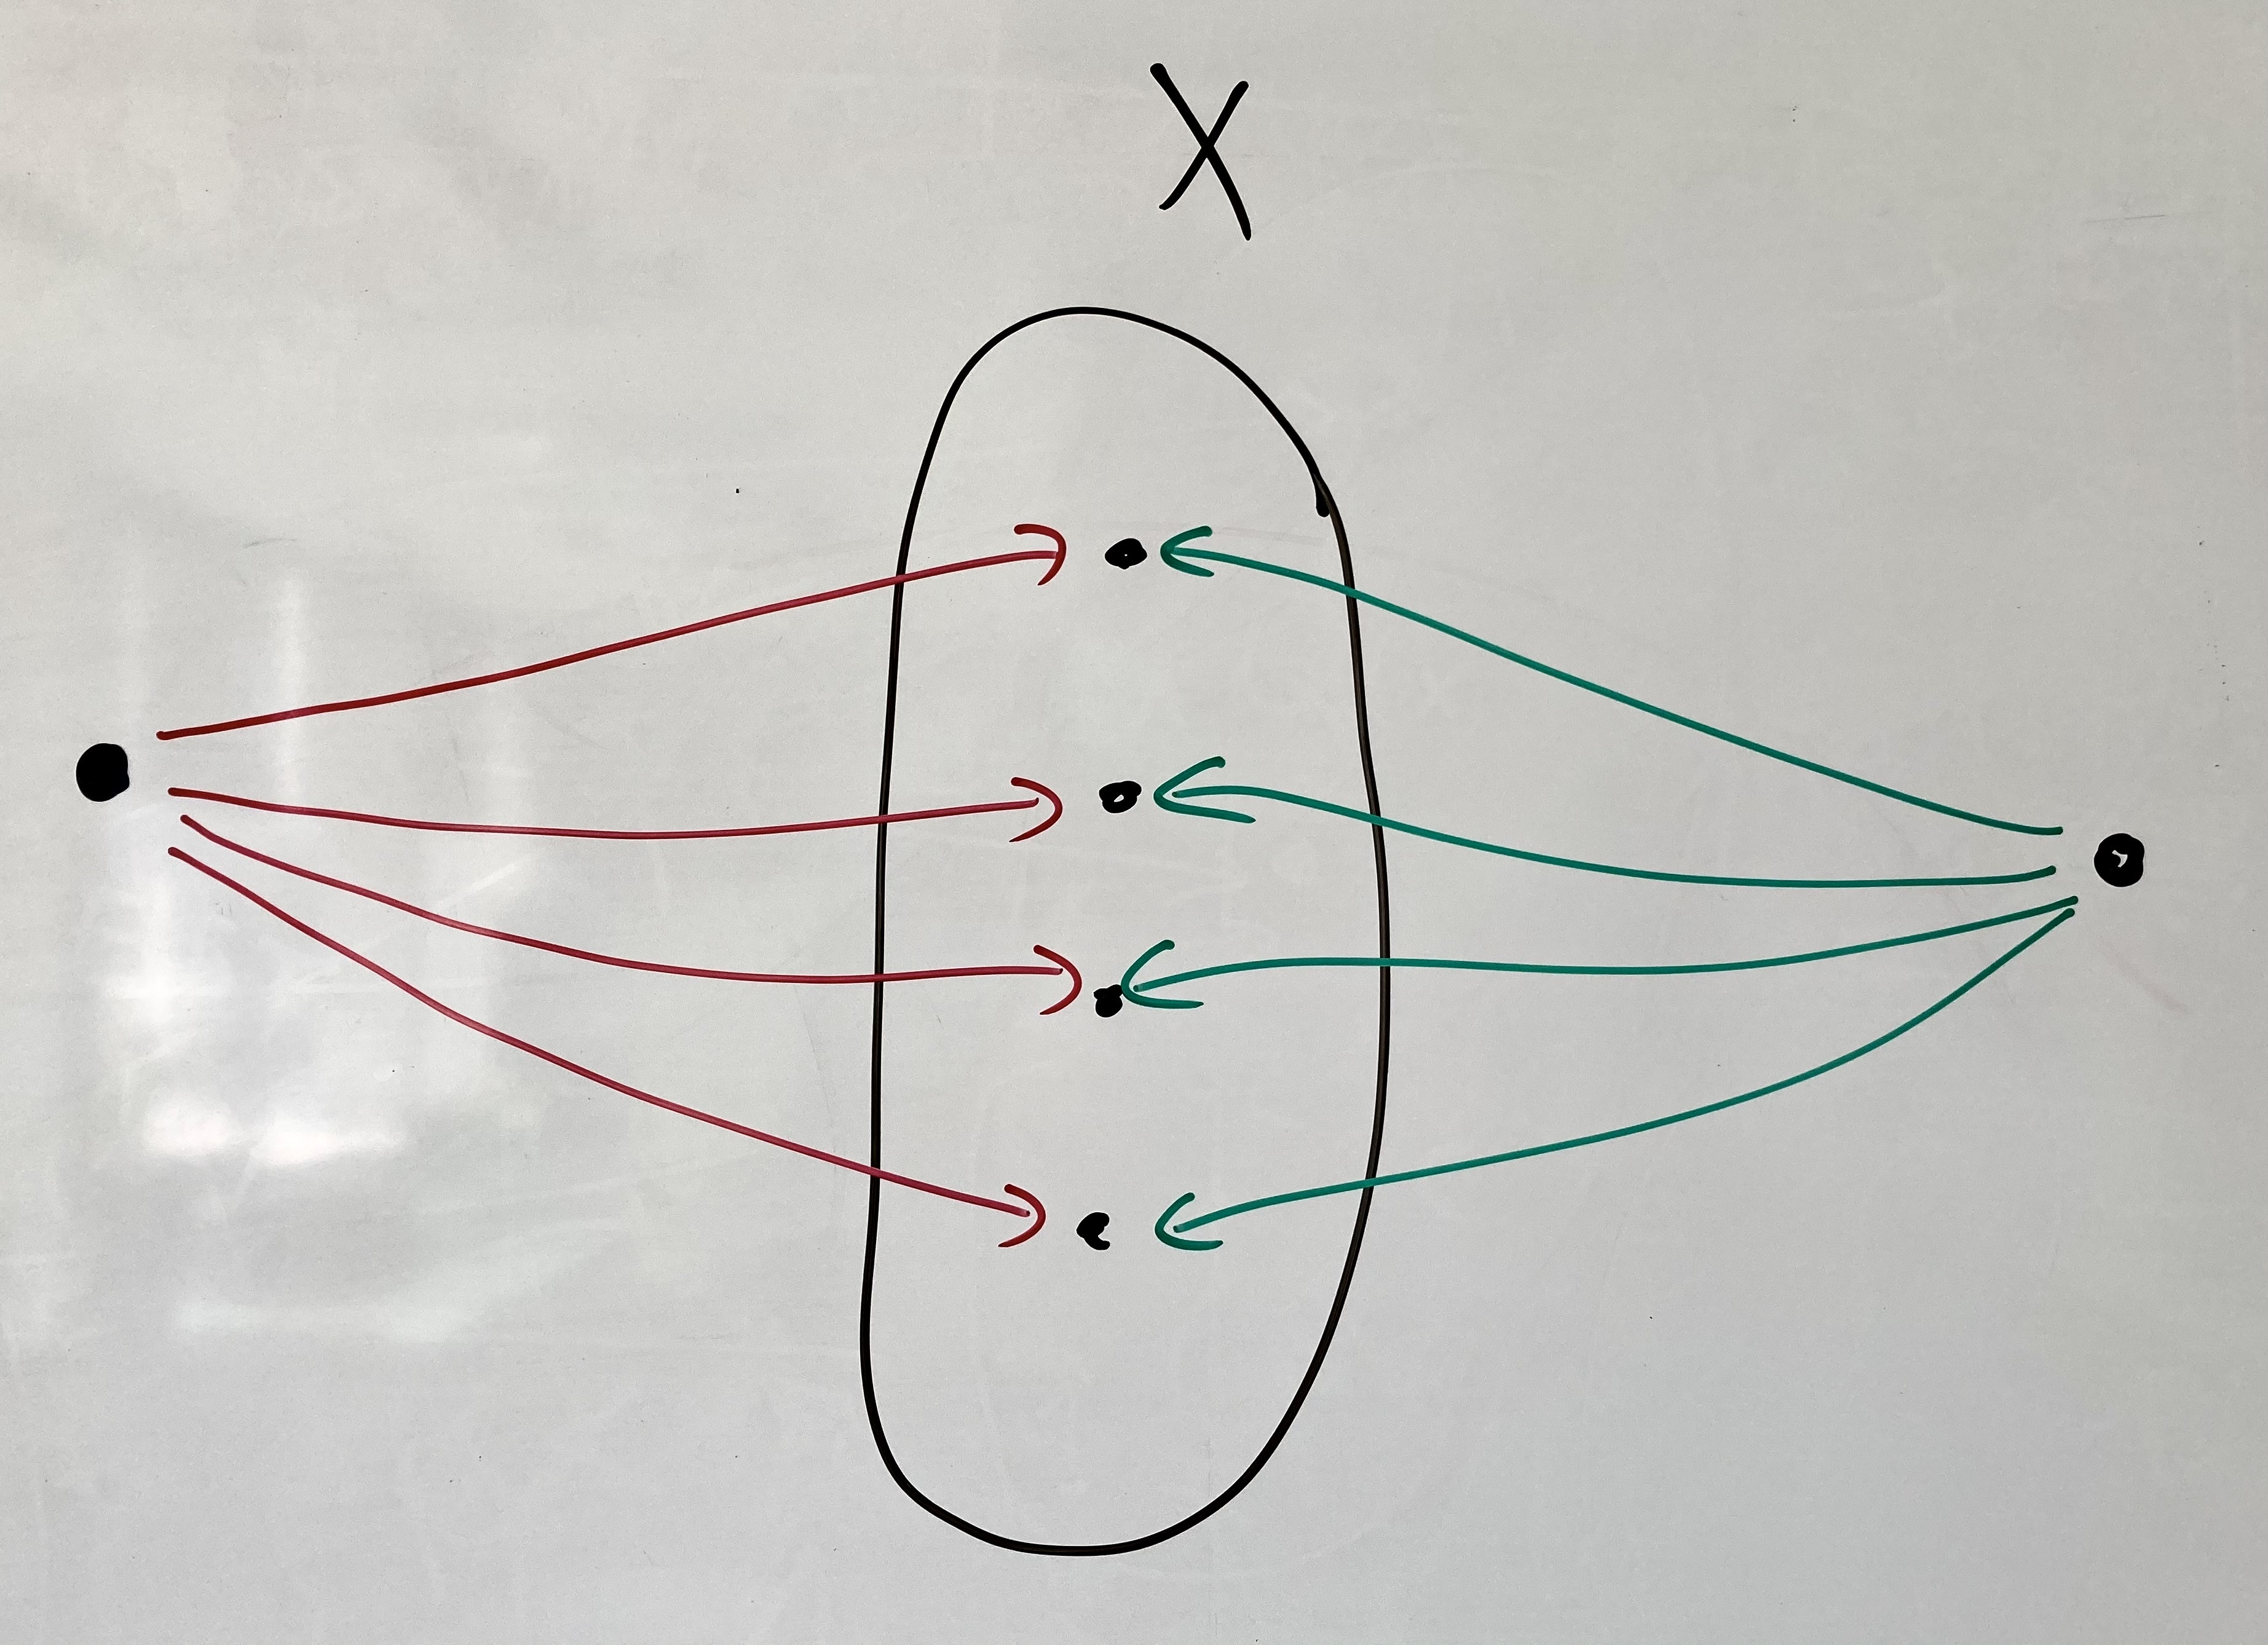
\includegraphics[width=.7\textwidth]{suspension-from-join-2}
  \end{center}
\end{frame}


\begin{frame}
  \begin{theorem}
    There is an equivalence $(A\ast B)\ast C\simeq A\ast(B\ast C)$. 
  \end{theorem}

  \begin{proof}
    By the 3-by-3 lemma.
  \end{proof}
  
  \begin{corollary}
    There is an equivalence $\sphere{n}\ast X\simeq \Sigma^{n+1}X$.
  \end{corollary}
  \begin{corollary}
    There is an equivalence $\sphere{n}\ast\sphere{m}\simeq \sphere{n+m+1}$. 
  \end{corollary}
\end{frame}

\begin{frame}
  \frametitle{Homotopy pullbacks}
  The notion of pullback is dual to the notion of pushout.
  \begin{definition}
    A commuting square
  \begin{equation*}
    \begin{tikzcd}[ampersand replacement=\&]
      C \arrow[d,swap,"p"] \arrow[r,"q"] \& B \arrow[d,"g"] \\
      A \arrow[r,swap,"f"] \& X,
    \end{tikzcd}
  \end{equation*}
  equipped with $H:f\circ p\sim g\circ q$ is said to be a \textbf{pullback square} if it satisfies the universal property of the pullback: For any type $C'$, the map
  \begin{equation*}
    (C'\to C)\to \sum_{(p':C'\to A)}\sum_{(q':C'\to B)}f\circ p'\sim g\circ q'
  \end{equation*}
  given by $h\mapsto (p\circ h,q\circ h,H\circ h)$, is an equivalence.
  \end{definition}
\end{frame}

\begin{frame}
  \frametitle{Existence of pullbacks}
  \begin{theorem}
    For any $A\stackrel{f}{\to} X \stackrel{g}{\leftarrow} B$, the square
    \begin{equation*}
      \begin{tikzcd}[ampersand replacement=\&]
        \sum_{(a:A)}\sum_{(b:B)}f(a)=g(b) \arrow[d] \arrow[r] \& B \arrow[d,"g"] \\
        A \arrow[r,swap,"f"] \& X
      \end{tikzcd}
    \end{equation*}
    is a pullback square.
  \end{theorem}

  \begin{proof}
    The universal property holds because $\Pi$ distributes over $\Sigma$:
    \begin{equation*}
      \left(X\to \sum_{(a:A)}\sum_{(b:B)}f(a)=g(b)\right)\simeq\sum_{(p':X\to A)}\sum_{(q':X\to B)}f\circ p'\sim g\circ q'.\qedhere
    \end{equation*}
  \end{proof}
\end{frame}

\begin{frame}
  Recall that the fiber of a map $f:A\to B$ at $b:B$ is defined as
  \begin{equation*}
    \fib_f(b):=\sum_{(a:A)}f(a)=b.
  \end{equation*}

  \begin{corollary}
    For any $f:A\to B$ and any $b:B$ we have a pullback square
    \begin{equation*}
      \begin{tikzcd}[ampersand replacement=\&]
        \fib_f(b) \arrow[d] \arrow[r,"\pi_1"] \& A \arrow[d,"f"] \\
        \unit \arrow[r] \& B
      \end{tikzcd}
    \end{equation*}
  \end{corollary}
\end{frame}

\begin{frame}
  \begin{theorem}
    Consider a commuting square
    \begin{equation*}
      \begin{tikzcd}[ampersand replacement=\&]
        E' \arrow[d,swap,"{p'}"] \arrow[r] \& E \arrow[d,"p"] \\
        B' \arrow[r,swap,"f"] \& B
      \end{tikzcd}
    \end{equation*}
    Then the following are equivalent:
    \begin{enumerate}
    \item The square is a pullback square.
    \item The induced map $\fib_{p'}(y)\to \fib_p(f(y))$ is an equivalence, for every $y:B'$.
    \end{enumerate}
  \end{theorem}
\end{frame}

\begin{frame}
  \begin{theorem}[Descent for pushouts]
    Consider a commuting cube
    \begin{equation*}
      \begin{tikzcd}[ampersand replacement=\&,row sep=small]
        \& S' \arrow[dl] \arrow[d] \arrow[dr] \\
        A' \arrow[d] \& S \arrow[dl] \arrow[dr] \& B' \arrow[dl,crossing over] \arrow[d] \\
        A \arrow[dr] \& X' \arrow[from=ul,crossing over] \arrow[d] \& B \arrow[dl] \\
        \& X
      \end{tikzcd}
    \end{equation*}
    In which the bottom square is a pushout square and the two vertical squares in the back are pullback squares. The following are equivalent:
    \begin{enumerate}
    \item The two vertical squares in the front are pullback squares.
    \item The top square is a pushout square.
    \end{enumerate}
  \end{theorem}
\end{frame}

\begin{frame}
  \frametitle{The Hopf fibration}
  Consider the following commuting cube:
  \begin{equation*}
    \begin{tikzcd}[ampersand replacement=\&,row sep=small]
      \& \sphere{1}\times\sphere{1} \arrow[dl,swap,"\pi_1"] \arrow[d,"\mu"] \arrow[dr,"\pi_2"] \\
      \sphere{1} \arrow[d] \& \sphere{1} \arrow[dl] \arrow[dr] \& \sphere{1} \arrow[dl,crossing over] \arrow[d] \\
      \unit \arrow[dr] \& \sphere{1}\ast\sphere{1} \arrow[from=ul,crossing over] \arrow[d,dashed] \& \unit \arrow[dl] \\
      \& \sphere{2}
    \end{tikzcd}
  \end{equation*}
  where $\mu$ is the complex multiplication constructed in lecture 5.1.
  \begin{itemize}
  \item The top and bottom squares are pushouts.
  \item The two back squares are pullback squares because
    \begin{equation*}
      \mu(x,\blank)\qquad\text{and}\qquad\mu(\blank,y)
    \end{equation*}
    are equivalences, for any $x,y:\sphere{1}$.
  \item Therefore the front two squares are pullbacks by the descent theorem.
  \end{itemize}
\end{frame}

\begin{frame}
  In particular, we have a pullback square
  \begin{equation*}
    \begin{tikzcd}[ampersand replacement=\&]
      \sphere{1} \arrow[r,"\inl"] \arrow[d] \& \sphere{1}\ast\sphere{1} \arrow[d] \\
      \unit \arrow[r] \& \sphere{2}.
    \end{tikzcd}
  \end{equation*}

  \begin{definition}
    We say that a composable pair of pointed maps $F\to E\to B$ between pointed types is a \textbf{fiber sequence} if it fits in a pullback square
    \begin{equation*}
      \begin{tikzcd}[ampersand replacement=\&]
        F \arrow[d] \arrow[r] \& E \arrow[d] \\
        \unit \arrow[r] \& B
      \end{tikzcd}
    \end{equation*}
  \end{definition}
\end{frame}

\begin{frame}
  In other words, we have a fiber sequence
  \begin{equation*}
    \begin{tikzcd}[ampersand replacement=\&]
      \sphere{1} \arrow[r] \& \sphere{1}\ast\sphere{1} \arrow[r] \& \sphere{2}
    \end{tikzcd}
  \end{equation*}
  Furthermore, we saw before that $\sphere{1}\ast\sphere{1}\simeq\sphere{3}$. Therefore we obtain a fiber sequence
  \begin{equation*}
    \begin{tikzcd}[ampersand replacement=\&]
      \sphere{1} \arrow[r] \& \sphere{3} \arrow[r,"h"] \& \sphere{2}.
    \end{tikzcd}
  \end{equation*}
  This fiber sequence is known as the \textbf{Hopf fibration}. There is only one higher Hopf fibration
  \begin{equation*}
    \begin{tikzcd}[ampersand replacement=\&]
      \sphere{3} \arrow[r] \& \sphere{7} \arrow[r,"h"] \& \sphere{4},
    \end{tikzcd}
  \end{equation*}
  which is related to the multiplication on $\sphere{3}$, inherited from the multiplication of the unit quaternions.
\end{frame}

\begin{frame}
  \frametitle{Exercises}
  \begin{enumerate}
  \item Let $P$ and $Q$ be propositions. Show that the join $P\ast Q$ is a proposition, and show that it satisfies the universal property of the disjunction $P\vee Q$, i.e., that
    \begin{equation*}
      (P\ast Q\to R)\to (P\to R)\times(Q\to R)
    \end{equation*}
    is an equivalence, for any proposition $R$.
  \item Let $P$ be a proposition. Show that the suspension $\Sigma P$ is a set, and show that
    \begin{equation*}
      (N=S)\simeq P.
    \end{equation*}
  \item Show that a type $A$ is a proposition if and only if the map
    \begin{equation*}
      \mathsf{inl} : A \to A\ast A
    \end{equation*}
    is an equivalence.
  \end{enumerate}
\end{frame}

\begin{frame}
  \textbf{Open problem:}\\
  Define the Grassmannians synthetically as higher inductive types.\\[\baselineskip]
  \textbf{Related open problem:}\\
  Find a pointed type $X$ such that $\Omega X\simeq \sphere{3}$.\\[\baselineskip]
  \textbf{Open "problem"}
  Find a way, if any, how $\Pi$ distributes over homotopy colimits.
\end{frame}

\end{document}
